\documentclass[a4paper,12pt]{article}
\setlength {\marginparwidth }{2cm}

% packages used
\usepackage{todonotes}
\usepackage{graphicx}
\usepackage{siunitx}

% titlepage information
\title{ZRecognition\\TPJ665\\Final Capstone Project}
\author{Patrick Ziajski \\ Zarak Khattak}
\date{\today}

\begin{document}

% titlepage
\maketitle
\vfill
\begin{center}
    \textbf{SENECA COLLEGE OF APPLIED ARTS AND TECHNOLOGY}\\School of Electronics and Mechanical Engineering Technology\\1750 Finch Ave East, Toronto, Ontario, M2J 2X5. Tel. 416-491-5050\\www.senecacollege.ca
\end{center}
\thispagestyle{empty}
\pagenumbering{roman}

% table of contents
\newpage
\tableofcontents

% main section
\newpage
\pagenumbering{arabic}
\section{Executive Summary}

\newpage
\section{Introduction}
Security is an important feature for a company providing a service to their customer. The company must ensure that its service can only be used by authorized personnel. This is where Z-Recognition comes into play. Z-Recognition is a license plate recognition system that ensures only authorized personnel have access to a designated area. Z-Recognition accomplishes this by taking an image of the approaching vehicle and processing it. If the vehicle is authorized, meaning the license plate is recognized, the vehicle is given access. Our group has decided on a license plate recognition system due to its uses in modern day society. Today, one can still find areas that are monitored by a single employee, or by a ticket-based entry system. These systems could be found inferior because of their reliance on periodic human interaction or supervision. Z-Recognition is designed to run autonomously with minimal costs, and a single requirement of an active internet. This license plate recognition system also implements a core feature in the future of computer technology, machine learning. With machine learning, an artificial intelligence (AI) can provide systems the ability to learn and improve without being explicitly programmed. This means that automated systems become more secure and reliable, without the need of constant supervision. Finally, this project will require both hardware and software implementation to be fully functional. It will require us to work with and learn both software development and hardware assembly which we, as Computer Engineering and Technology students, would prefer.

\newpage
\section{Functional Features}
\begin{itemize}
    \item Image processing - Using Microsoft's Cloud based Computer Vision Service, called Azure, a captured image will be uploaded to Azure's Service. The service perform Optical Character Recognition (OCR) on the image, and it will return a JavaScript Object Notation (JSON) object with all the recognized characters.
    \item Motor Control - The Raspberry Pi 3 Model B, a MicroController Unit (MCU), will control a servo-motor to imitate a gate arm used to allow entrance into a secure area.
    \item Scheduled script execution - The main python script will be executed at specified time intervals
    \item Sound execution - The Raspberry Pi will emit a sound from a speaker in order to audibly notify the personnel using the system of whether they have been given or denied access.
\end{itemize}

\newpage
\section{System Specifications}
Camera
\begin{itemize}
    \item 720p/30fps
    \item Fixed focus
    \item Field of View - \ang{60}
\end{itemize}
Raspberry Pi 3 Model B
\begin{itemize}
    \item Quad Core 1.2GHz Broadcom BCM2837 64bit CPU
    \item 1GB RAM
    \item BCM43438 wireless LAN
    \item 40-pin extended GPIO
    \item 4 Pole stereo output
    \item Micro SD
\end{itemize}
Servo-motor
\begin{itemize}
    \item Operating voltage - 3.0V ~ 7.2V
\end{itemize}
Microsoft Azure
\begin{itemize}
    \item Active subscription
    \item Cognitive Services resource
\end{itemize}

\newpage
\section{Product Design, Implementation, and Operation of the System}
\subsection{System block-diagram}
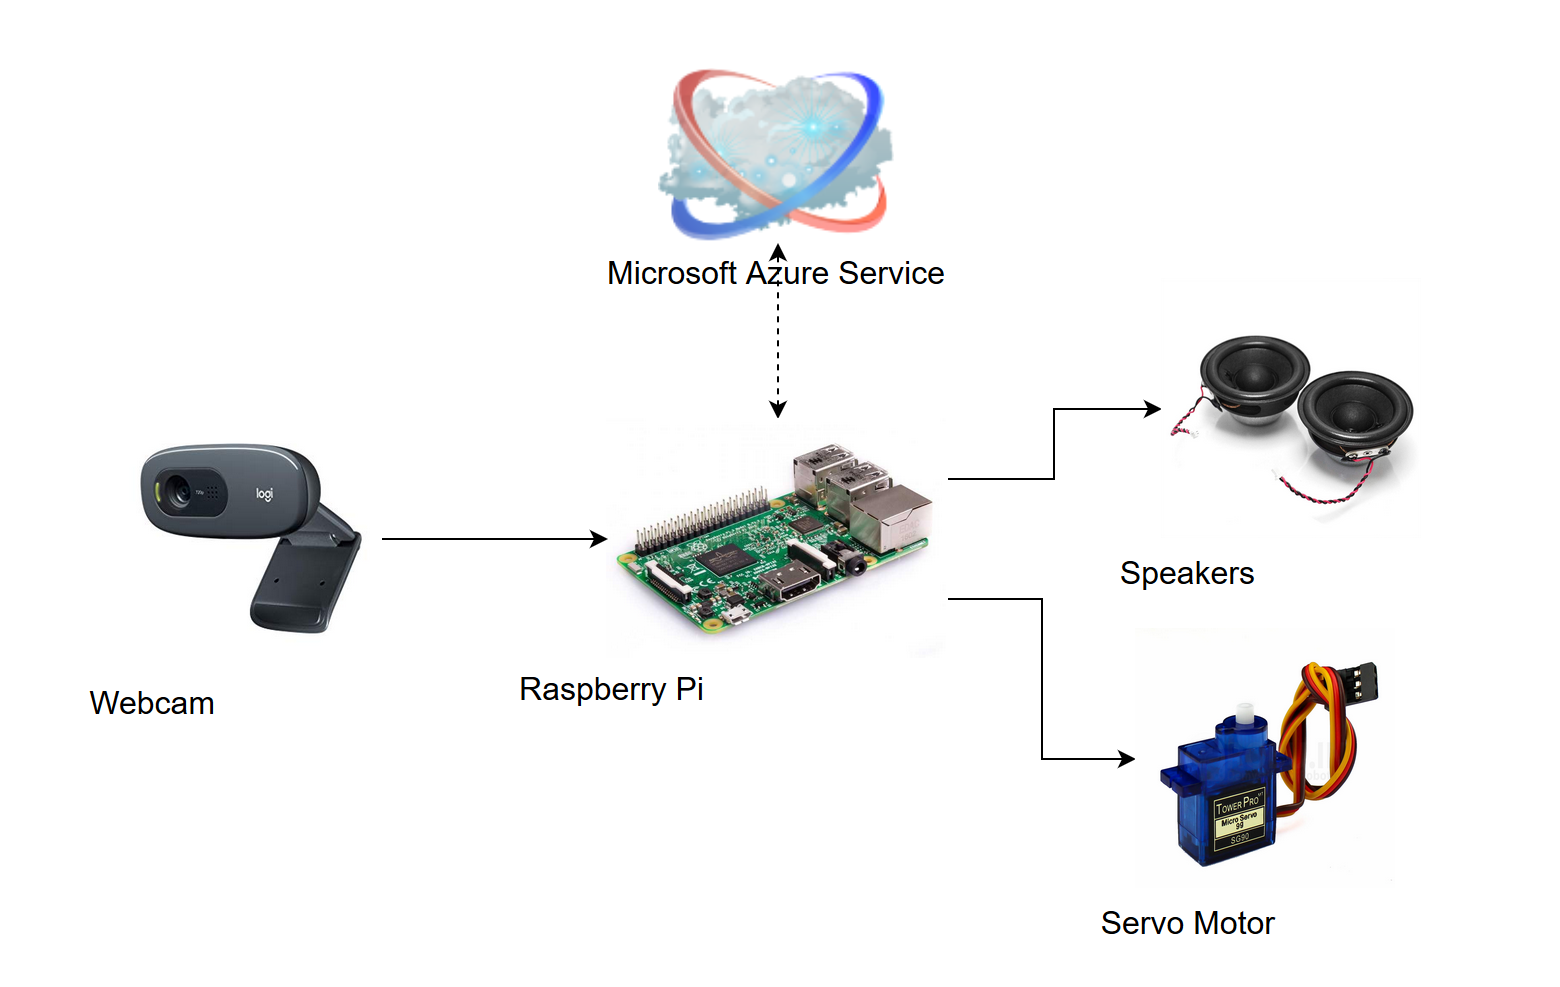
\includegraphics[width = \linewidth]{../images/BlockDiagram.png}
\subsection{UML diagram}
\subsection{Software flow-chart}
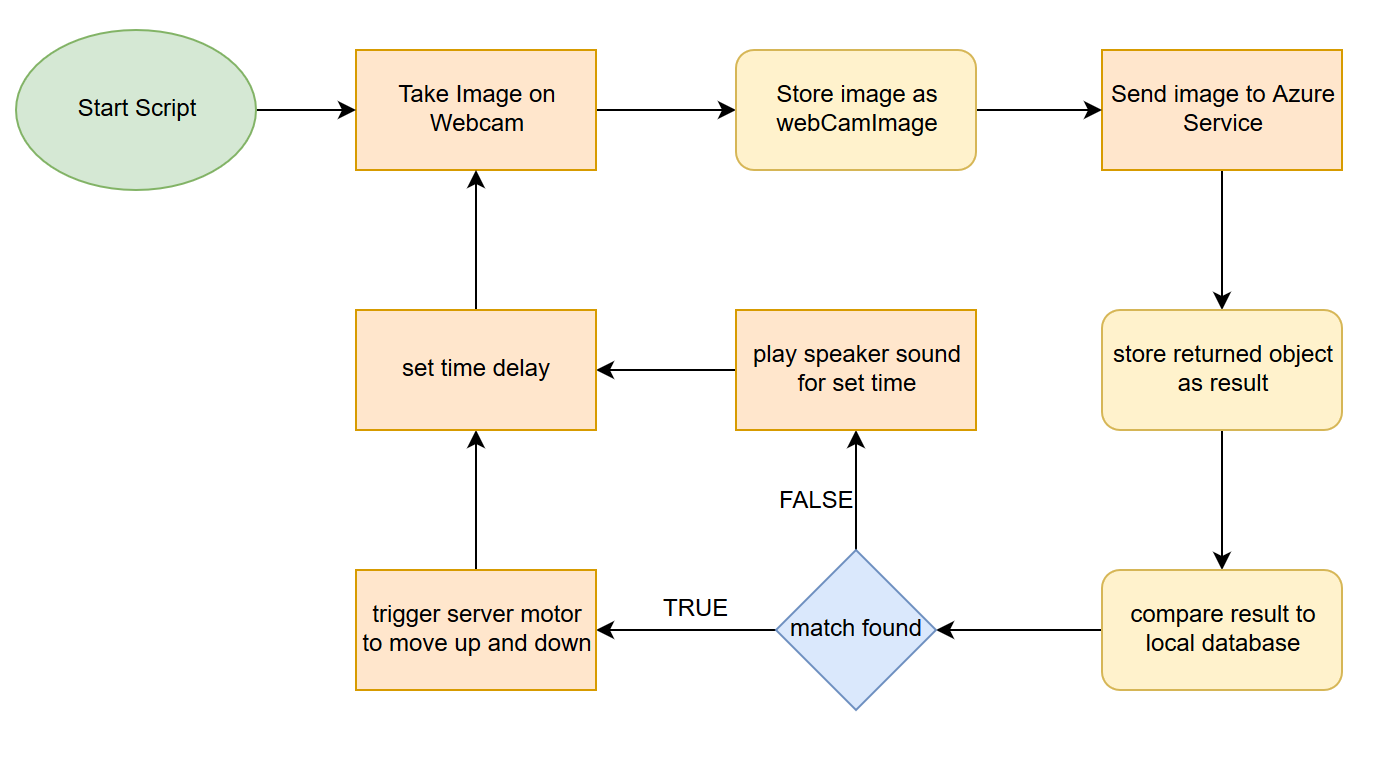
\includegraphics[width = \linewidth]{../images/FlowChart.png}
% \subsection{Component images and components description/Captures of the major GUI used}
\subsection{Theory of operation of the entire system}

% appendix
\newpage
\appendix
\section{Electrical Schematics}
\section{Parts List}
\section{References}

\newpage
\section{Contact Information}
\begin{center}
    Patrick Ziajski \\*
    Phone: (647) 339 2847 \\*
    Email: pziajski@myseneca.ca \\
    \vspace{5mm}
    Zarak Khattak \\*
    Phone: \todo{add phone number}\\*
    Email: zkhattak@myseneca.ca
\end{center}

% \section{Description of the attached CD content}

\end{document}